% !TeX root = ../thuthesis-example.tex

\chapter{新 \emph{insertRecords} 写入机制总体设计}
本章介绍新 \emph{insertRecords} 写入机制的总体设计,包括客户端侧数据预处理、RPC 数据序列化格式设计、存储引擎批量并行化写入。

\section{新写入设计总览}
\begin{figure}
  \centering
  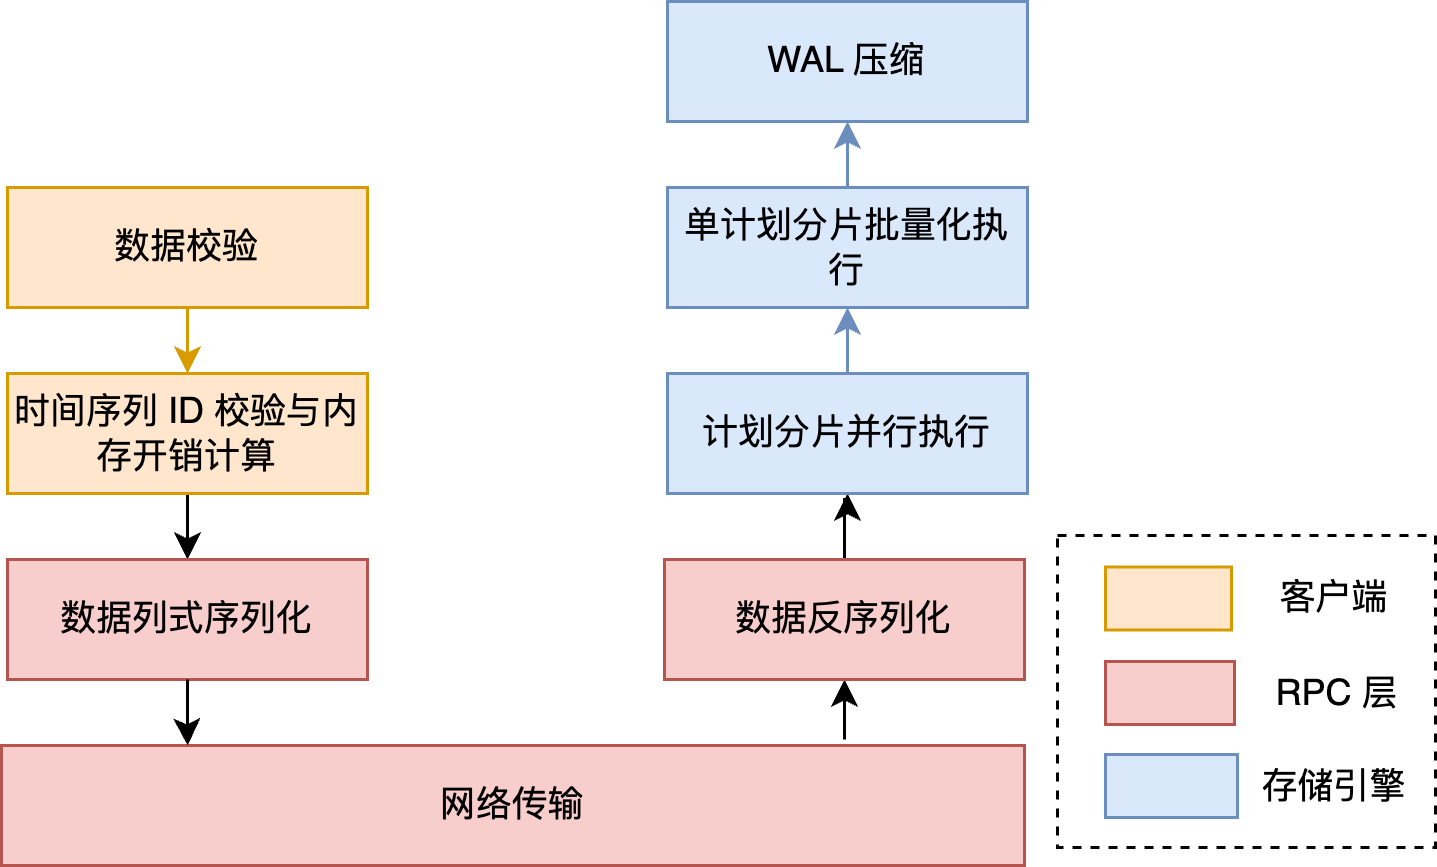
\includegraphics[width=\linewidth]{new-insert-records-overview.png}
  \caption{新 \emph{insertRecords} 写入机制}
  \label{fig:new-insert-records-overview}
\end{figure}

图 \ref{fig:new-insert-records-overview} 展示了新 \emph{insertRecords} 写入机制的总体设计。新写入机制有如下的设计目标:
\begin{enumerate}
  \item 提高系统性能:在相同的硬件下实现更高的写入性能,包括更高的吞吐以及更低的延迟;或者在相同的写入性能下降低对系统资源的使用;
  \item 提高系统整体资源的利用率:充分利用系统中客户端和服务器侧的计算、存储、网络资源,避免资源闲置;
  \item 具有高稳定性:在持续的高负载下系统应当能够保持较好的写入性能,避免出现剧烈的波动。
\end{enumerate}
为了实现这样的目标,新写入机制的总体设计思路为:
\begin{itemize}
  \item 存储引擎侧构建高效率的写入方式,将数据批量化、并行化写入,将写入过程中的固定开销尽量平摊到多条数据上,提高系统资源的利用率。
  \item 将服务器端的部分工作卸载(Offload)到客户端上,在客户端侧进行少量轻量级的计算,提高整体资源的利用率。
  \item 减少经过网络传输的冗余数据量,通过高效的列式数据格式提高网络资源的利用率。
\end{itemize}
本章的剩余内容从客户端、RPC 层、存储引擎三个方面简要介绍新 \emph{insertRecords} 写入机制的设计。

\section{客户端侧数据预处理}
在 \ref{sec:chap2-sec3} 节中,本文介绍了一些对于客户端进行优化的相关工作。其中, Crystal 存储系统基于远程存储所设计\cite{durner2021crystal}。因为数据通过远程存储设施进行读取的性能较差,所以为了提高系统的性能,Crystal 的客户端增加了谓词下推功能,被下推到数据源的谓词可以提前过滤掉一些不符合条件的数据,减少通过网络传输的数据量,提高系统的性能。在时序数据库中,TDEngine 的客户端也是“重客户端”设计的代表。TDEngine 的客户端不仅承担了对 SQL 进行解析的工作,还负责缓冲系统的元数据,在写入之前进行元数据校验。

目前 IoTDB 的客户端只负责数据的简单校验和传输,其余工作都由服务器承担。从系统的整体资源利用率的角度看,在目前的设计中 IoTDB 客户端侧的资源并没有被充分利用起来。因此,本文将服务器所承担的部分不依赖于已有数据的工作卸载到客户端侧。参考表 \ref{tabular:insert-records-profile-result} 可知,这一类工作中开销最大的就是时间序列 ID 和内存开销计算,本工作将会把这两项任务从服务器端移到客户端。

\section{写入请求列式序列化}
IoTDB 是一个时序数据库,本质上是一个针对时序场景优化的 OLAP 数据库\cite{谭新宇2023一致性协议}。在 OLAP 数据库中提高系统性能的一个常见方式是将数据按照列的形式存储和处理。根据 \ref{sec:chap3-sec2} 的对目前 IoTDB \emph{insertRecords} 写入请求序列化的介绍可以知道,目前所使用的序列化方式是行式的。结合 \ref{sec:chap3-sec3-1} 节的实验结果,可以得出目前行式序列化出来的写入请求较大,进而导致在实验环境下网络资源紧张的结论。为了解决这一问题,设计一个列式的数据序列化格式,并结合列式存储中常用的编码(Encode)、压缩(Compress)等技术,降低写入请求序列化后的体积。

正如 \ref{sec:chap2-sec3} 节中所述,设计序列化格式是一个需要权衡的过程,追求过小的数据包体积可能导致序列化和反序列化的开销过大,追求较低的序列化和反序列化开销则可能导致序列化得到的数据包体积过大。此外,由于 IoTDB 使用 Java 编写,数据序列化和反序列化对内存垃圾回收(Garbage Collection,GC)造成的影响也是我们需要考虑的重要因素。为了兼顾以上的因素,本文实现了一种可以根据系统当前负载状况动态使用压缩与编码的写入请求序列化方法。

\section{存储引擎侧批量并行化写入}
数据库系统高性能写入的实现离不开高性能存储引擎的支持。结合 \ref{sec:chap3-sec2} 节与 \ref{sec:chap3-sec3-1} 节的内容,IoTDB 存储引擎对 \emph{insertRecords} 写入实现最大的缺陷是没有做到批量化执行,造成了一些非核心流程的开销过大。因此,新 \emph{insertRecords} 写入机制在存储引擎侧执行写入请求时会将多条记录一齐写入到内存表中,在写入的过程中集中序列化写前日志、更新内存缓存、记录系统监控,避免多次调用这些非核心流程,通过统一调用来将它们的开销平摊到多条记录上。

以上的批量化写入是在计划分片(FragmentInstance,FI)级别的,而在 \ref{sec:chap3-sec2} 节的写入流程中,写入本地多个 DataRegion 的计划分片是串行执行的。当系统的负载不高时,这样串行执行并不能充分利用系统的资源。并且,由于后续分片的执行需要等待前序分片都执行完毕了才可以开始,写入的延迟也会提高。所以,本文将写入本地分片的过程并行化,以充分利用服务器多 CPU 核心的潜力。

在 \ref{sec:chap3-sec3-1} 节的实验结果中,\emph{insertRecords} 写入所产生的写前日志体积超过了最终 TsFile 体积的 7 倍,这不是一种合理的现象,大量的写前日志会占据系统的 I/O、内存和 CPU 资源。为了解决这一现象,新 \emph{insertRecords} 写入机制对写入同一 DataRegion 下的记录集中序列化写前日志,并且对写前日志采用轻量化的压缩算法进行压缩,显著地减少了写前日志的大小。

\section{本章小结}
本章简要介绍了新 \emph{insertRecords} 写入机制的设计目标与设计思路,以及对客户端、RPC 层、存储引擎的设计要点,让读者从全局的视角了解本文的优化工作。后文将分别从客户端、RPC 层以及存储引擎三个角度深入地介绍每一项优化工作。